\section{Mikrokontroler}
\label{sec:konsep-mikrokontroler}

\begin{wrapfigure}{r}{0.38\textwidth} % 'r' = sisi kanan, 0.38\textwidth = lebar area gambar
	\vspace{-12pt} % Menggeser posisi gambar sedikit ke atas agar sejajar dengan baris pertama teks
	\centering
	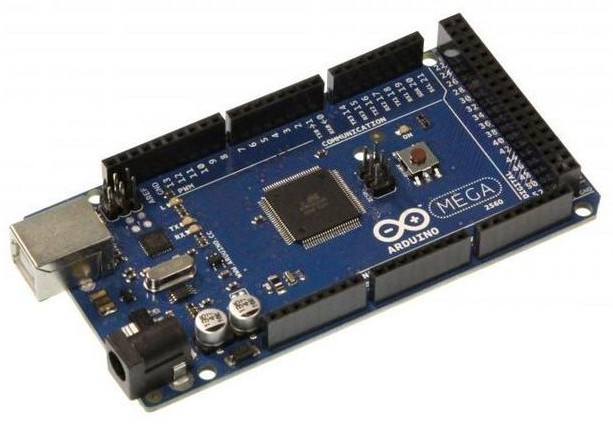
\includegraphics[width=0.36\textwidth]{images/2560.jpg} % Ganti dengan file gambar Anda
	\caption{Ardunio ATmega2560}
	\label{fig:pembuka_mcu}
	\vspace{-10pt} % Mengurangi jarak kosong di bawah caption
\end{wrapfigure}

Bagian ini memberikan landasan konseptual mengenai mikrokontroler sebelum pembahasan masuk ke prinsip kerja masing-masing komponen. Mikrokontroler berperan sebagai pusat pengendalian yang membaca masukan, memproses data, dan menghasilkan keluaran sesuai program. Pemahaman mengenai konsep ini diperlukan agar hubungan antara karakteristik komponen dan fitur mikrokontroler dapat dijelaskan secara teknis.

\par % Memastikan paragraf tersusun rapi sebelum masuk ke subbab berikutnya

\subsection{Pengertian dan Peran Mikrokontroler}
Mikrokontroler adalah sebuah sistem komputer lengkap yang dikemas dalam satu sirkuit terpadu (\textit{Integrated Circuit}/IC). Berbeda dengan mikroprosesor umum (seperti CPU pada PC) yang membutuhkan komponen eksternal terpisah seperti RAM, ROM, dan pengontrol I/O, mikrokontroler telah mengintegrasikan pemroses, memori, dan antarmuka periferal ke dalam satu cip tunggal.

Dalam sistem deteksi udara dan gas pada kegiatan ini, mikrokontroler beroperasi sebagai unit pemroses terpusat (\textit{brain module}). Mikrokontroler bertugas membaca sinyal fisik dari sensor (seperti suhu, gas, dan gerakan), memproses data tersebut berdasarkan algoritma kendali, lalu memberikan instruksi kepada aktuator (seperti penggerak servo, motor DC, atau sakelar relay) untuk merespons kondisi lingkungan secara akurat.

\begin{figure}[H]
	\centering
	\resizebox{\textwidth}{!}{%
		\begin{tikzpicture}[
				node distance=0.6cm and 0.25cm,
				block/.style={rectangle, draw, fill=blue!10, rounded corners=2pt, minimum width=2.1cm, minimum height=1.1cm, align=center, font=\small\sffamily\bfseries},
				core/.style={rectangle, draw, fill=red!15, minimum width=3.2cm, minimum height=1.1cm, align=center, font=\small\sffamily\bfseries},
				arrow/.style={Latex-Latex, thick, draw=gray!80}
			]

			% 1. Buat 6 Blok Bawah Terlebih Dahulu secara Sejajar Horisontal
			\node[block] (eeprom) {EEPROM\\(4 KB)};
			\node[block, right=0.25cm of eeprom] (sram) {SRAM\\(8 KB)};
			\node[block, right=0.25cm of sram] (flash) {Flash Memory\\(256 KB)};
			\node[block, right=0.25cm of flash] (gpio) {GPIO / Pin I/O\\(54 Pin)};
			\node[block, right=0.25cm of gpio] (adc) {ADC 10-bit\\(16 Saluran)};
			\node[block, right=0.25cm of adc] (comm) {Komunikasi\\UART / SPI / I2C};

			% 2. Gambar Bus Abu-Abu Presisi dari Ujung Kiri EEPROM ke Ujung Kanan COMM
			\draw[fill=gray!30, draw=black]
			($(eeprom.north west)+(0, 0.6cm)$) rectangle ($(comm.north east)+(0, 1.05cm)$);

			% Tulis Teks di Tengah Bus
			\path ($(eeprom.north west)!0.5!(comm.north east)+(0, 0.825cm)$)
			node[font=\small\sffamily\bfseries] (bus_text) {BUS DATA \& ALAMAT INTERNAL};

			% Koordinat Sisi Atas dan Bawah Bus untuk Acuan Panah
			\coordinate (bus_south) at ($(eeprom.north west)+(0, 0.6cm)$);
			\coordinate (bus_north) at ($(eeprom.north west)+(0, 1.05cm)$);

			% 3. Buat CPU di Atas Bus (Tepat di Tengah Horisontal)
			\node[core, above=0.7cm of bus_text.north] (cpu) {CPU (8-bit AVR)\\Unit Pemroses Utama};

			% 4. Tarik Panah Hubungan
			\draw[arrow] (cpu.south) -- (cpu.south |- bus_north);
			\draw[arrow] (eeprom.north) -- (eeprom.north |- bus_south);
			\draw[arrow] (sram.north) -- (sram.north |- bus_south);
			\draw[arrow] (flash.north) -- (flash.north |- bus_south);
			\draw[arrow] (gpio.north) -- (gpio.north |- bus_south);
			\draw[arrow] (adc.north) -- (adc.north |- bus_south);
			\draw[arrow] (comm.north) -- (comm.north |- bus_south);

		\end{tikzpicture}%
	}
	\caption{Diagram blok arsitektur dasar mikrokontroler ATmega2560.}
	\label{fig:mcu_architecture}
\end{figure}

\subsection{General Purpose Input/Output (GPIO) dan Logika Digital}

Pin \textit{General Purpose Input/Output} (GPIO) merupakan antarmuka diskrit pada mikrokontroler yang arah operasinya dikonfigurasi via perangkat lunak melalui \textit{Data Direction Register} (DDR). Saat memproses sinyal biner, GPIO bekerja pada dua taraf logika:
\begin{itemize}
    \item \textbf{Logika HIGH (1):} Sinyal aktif ketika tegangan berada pada ambang atas mendekati $V_{CC}$ ($\approx 5\,\text{V DC}$).
    \item \textbf{Logika LOW (0):} Sinyal non-aktif ketika tegangan berada pada ambang bawah mendekati \textit{Ground} ($0\,\text{V DC}$).
\end{itemize}

\subsubsection{Kondisi Mengambang (\textit{Floating State}) dan Resistor Pembatas}

Saat dikonfigurasi sebagai \textit{input}, gerbang internal GPIO berada pada kondisi impedansi tinggi (\textit{High-Z}, $>100\,\text{M}\Omega$). Jika sakelar atau sensor di luarnya terbuka (\textit{open circuit}), pin masukan terisolasi dari tegangan maupun \textit{Ground}. Kondisi ini membuat pin bertindak seperti antena yang rentan terhadap induksi elektromagnetik dan \textit{noise} lingkungan, sehingga tegangannya berfluktuasi acak antara $0\,\text{V}$ dan $5\,\text{V}$ (\textit{floating state}).

Fluktuasi akibat \textit{floating} dapat memicu interupsi palsu (\textit{glitch}) dan kesalahan logika program. Oleh karena itu, sistem memerlukan kepastian status sinyal saat tidak ada masukan aktif. Kepastian logika ini dicapai melalui teknik \textit{biasing} menggunakan resistor (umumnya $10\,\text{k}\Omega$) dalam dua skema:
\begin{itemize}
    \item \textbf{Resistor \textit{Pull-Up}:} Menghubungkan pin masukan ke $V_{CC}$. Saat sakelar terbuka, pin ditarik ke $V_{CC}$ (\texttt{HIGH}). Ketika sakelar ditutup ke \textit{Ground}, tegangan pin jatuh ke $0\,\text{V}$ (\texttt{LOW}) tanpa menyebabkan hubung singkat.
    \item \textbf{Resistor \textit{Pull-Down}:} Menghubungkan pin masukan ke \textit{Ground}. Saat sakelar terbuka, pin ditarik ke \textit{Ground} (\texttt{LOW}). Ketika sakelar ditutup ke $V_{CC}$, pembacaan pin berubah menjadi \texttt{HIGH}.
\end{itemize}

Pada Arduino Mega 2560 (ATmega2560), setiap pin GPIO telah memiliki \textit{Internal Pull-Up Resistor} ($20\text{--}50\,\text{k}\Omega$) yang dapat diaktifkan melalui register perangkat lunak, sehingga menyederhanakan rangkaian eksternal.

\subsection{ADC dan Pembacaan Sinyal Analog}
\textit{Analog-to-Digital Converter} (ADC) berfungsi mengubah sinyal tegangan kontinu dari sensor analog menjadi nilai digital diskrit. Mikrokontroler ATmega2560 dilengkapi dengan ADC beresolusi $10\text{-bit}$ dan tegangan referensi standar $V_{ref} = 5\,\text{V}$.

Sinyal tegangan masuk $V_{in}$ dikonversi menjadi nilai digital $D_{out}$ bertipe integer ($0$ hingga $2^{10}-1 = 1023$) berdasarkan Persamaan~\eqref{eq:adc_conversion}:

\begin{equation}
	\label{eq:adc_conversion}
	D_{out} = \left\lfloor \frac{V_{in}}{V_{ref}} \times (2^n - 1) \right\rfloor = \left\lfloor \frac{V_{in}}{5\,\text{V}} \times 1023 \right\rfloor
\end{equation}

Sebagai contoh, jika sensor MQ-135 menghasilkan tegangan keluaran analog sebesar $2{,}5\,\text{V}$, maka nilai digital yang dibaca oleh ADC mikrokontroler adalah:
\[
	D_{out} = \left\lfloor \frac{2{,}5\,\text{V}}{5\,\text{V}} \times 1023 \right\rfloor = 511
\]

\subsection{PWM dan Pengendalian Output}
\textit{Pulse Width Modulation} (PWM) adalah teknik untuk menyimulasikan luaran analog menggunakan sinyal digital cepat berfrekuensi tetap. Parameter utama PWM adalah \textit{Duty Cycle}, yaitu rasio durasi sinyal \textit{HIGH} ($t_{on}$) terhadap total periode sinyal ($T$), dirumuskan pada Persamaan~\eqref{eq:duty_cycle}:

\begin{equation}
	\label{eq:duty_cycle}
	\text{Duty Cycle (\%)} = \left( \frac{t_{on}}{T} \right) \times 100\%
\end{equation}

Tegangan efektif rata-rata ($V_{eff}$) yang diterima oleh beban dirumuskan pada Persamaan~\eqref{eq:v_eff}:

\begin{equation}
	\label{eq:v_eff}
	V_{eff} = V_{CC} \times \text{Duty Cycle}
\end{equation}

Ilustrasi bentuk gelombang sinyal PWM pada berbagai variasi \textit{duty cycle} disajikan pada Gambar~\ref{fig:pwm_waveform}.

\begin{figure}[H]
	\centering
	\resizebox{0.85\textwidth}{!}{%
		\begin{tikzpicture}[
				xscale=1.6, yscale=0.85,
				signal/.style={ultra thick, blue!80!black},
				avg/.style={dashed, red!80!black, thick}
			]

			% ==================== 1. DUTY CYCLE 25% ====================
			\begin{scope}[shift={(0,5.6)}]
				% Judul Tanpa Label A/B/C
				\node[anchor=west, font=\scriptsize\sffamily\bfseries] at (0.2, 2.3) {Duty Cycle 25\% ($V_{eff} = 0.25 \, V_{CC}$)};

				% Sumbu Koordinat
				\draw[-Latex, thick] (-0.1,0) -- (4.3,0) node[right, font=\small\sffamily] {$t$};
				\draw[-Latex, thick] (0,-0.15) -- (0,2.1) node[above, font=\small\sffamily] {$V$};

				% Label Sumbu Tegangan (Presisi di Samping Sumbu Y)
				\node[anchor=east, font=\tiny] at (-0.08, 1.8) {$V_{CC}$};
				\node[anchor=east, font=\tiny] at (-0.08, 0) {$0\text{V}$};

				% Gelombang Pulsa
				\draw[signal] (0,0) -- (0,1.8) -- (0.5,1.8) -- (0.5,0) -- (2,0) -- (2,1.8) -- (2.5,1.8) -- (2.5,0) -- (4,0);

				% Garis Rata-rata Veff
				\draw[avg] (0,0.45) -- (4,0.45) node[right, font=\tiny\sffamily, red!80!black] {$V_{eff}$};

				% Indikator Ton
				\draw[Latex-Latex, thin] (0,1.3) -- (0.5,1.3) node[midway, above=-2pt, font=\tiny] {$t_{on}$};
			\end{scope}

			% ==================== 2. DUTY CYCLE 50% ====================
			\begin{scope}[shift={(0,2.8)}]
				% Judul Tanpa Label A/B/C
				\node[anchor=west, font=\scriptsize\sffamily\bfseries] at (0.2, 2.3) {Duty Cycle 50\% ($V_{eff} = 0.50 \, V_{CC}$)};
				% Sumbu Koordinat
				\draw[-Latex, thick] (-0.1,0) -- (4.3,0) node[right, font=\small\sffamily] {$t$};
				\draw[-Latex, thick] (0,-0.15) -- (0,2.1) node[above, font=\small\sffamily] {$V$};

				% Label Sumbu Tegangan
				\node[anchor=east, font=\tiny] at (-0.08, 1.8) {$V_{CC}$};
				\node[anchor=east, font=\tiny] at (-0.08, 0) {$0\text{V}$};

				% Gelombang Pulsa
				\draw[signal] (0,0) -- (0,1.8) -- (1,1.8) -- (1,0) -- (2,0) -- (2,1.8) -- (3,1.8) -- (3,0) -- (4,0);

				% Garis Rata-rata Veff
				\draw[avg] (0,0.9) -- (4,0.9) node[right, font=\tiny\sffamily, red!80!black] {$V_{eff}$};

				% Indikator Ton
				\draw[Latex-Latex, thin] (0,1.3) -- (1,1.3) node[midway, above=-2pt, font=\tiny] {$t_{on}$};
			\end{scope}

			% ==================== 3. DUTY CYCLE 75% ====================
			\begin{scope}[shift={(0,0)}]
				% Judul Tanpa Label A/B/C
				\node[anchor=west, font=\scriptsize\sffamily\bfseries] at (0.2, 2.3) {Duty Cycle 75\% ($V_{eff} = 0.75 \, V_{CC}$)};

				% Sumbu Koordinat
				\draw[-Latex, thick] (-0.1,0) -- (4.3,0) node[right, font=\small\sffamily] {$t$};
				\draw[-Latex, thick] (0,-0.15) -- (0,2.1) node[above, font=\small\sffamily] {$V$};


				% Label Sumbu Tegangan
				\node[anchor=east, font=\tiny] at (-0.08, 1.8) {$V_{CC}$};
				\node[anchor=east, font=\tiny] at (-0.08, 0) {$0\text{V}$};

				% Gelombang Pulsa
				\draw[signal] (0,0) -- (0,1.8) -- (1.5,1.8) -- (1.5,0) -- (2,0) -- (2,1.8) -- (3.5,1.8) -- (3.5,0) -- (4,0);

				% Garis Rata-rata Veff
				\draw[avg] (0,1.35) -- (4,1.35) node[right, font=\tiny\sffamily, red!80!black] {$V_{eff}$};

				% Indikator Ton
				\draw[Latex-Latex, thin] (0,1.3) -- (1.5,1.3) node[midway, above=-2pt, font=\tiny] {$t_{on}$};

				% Indikator Periode T
				\draw[Latex-Latex, thin] (0,-0.55) -- (2,-0.55) node[midway, below=-1pt, font=\tiny] {Periode ($T$)};
				\draw[dotted, gray] (2,0) -- (2,-0.55);
				\draw[dotted, gray] (0,0) -- (0,-0.55);
			\end{scope}

		\end{tikzpicture}%
	}
	\caption{Bentuk gelombang sinyal PWM pada variasi \textit{duty cycle} 25\%, 50\%, dan 75\% beserta tegangan efektif rata-ratanya ($V_{eff}$).}
	\label{fig:pwm_waveform}
\end{figure}

PWM digunakan secara mendasar dalam eksperimen ini untuk mengendalikan posisi sudut servo SG90 (lebar pulsa $1\text{--}2\,\text{ms}$) serta mengatur kecepatan putar Motor DC melalui rasio tegangannya.

\subsection{Timer dan Interrupt}
\begin{itemize}
	\item \textbf{Timer/Counter:} Periferal independen dari CPU yang menghitung pulsa detak mikrokontroler. Timer memungkinkan pewaktuan presisi tanpa membebani CPU (\textit{non-blocking delay}).
	\item \textbf{Interrupt:} Mekanisme yang menghentikan sementara eksekusi program utama (\textit{main loop}) ketika terjadi peristiwa tertentu (misalnya perubahan logika pin atau limpahan timer/overflow). CPU akan melompat ke fungsi khusus yang disebut \textit{Interrupt Service Routine} (ISR), mengeksekusinya, lalu kembali ke alur program utama. Mekanisme ini sangat krusial untuk menangani interupsi darurat dari sensor krisis seperti deteksi gas berlebih atau sensor pergerakan PIR.
\end{itemize}

\subsection{Antarmuka Komunikasi}
Mikrokontroler memanfaatkan beberapa protokol komunikasi serial terstandar:
\begin{itemize}
	\item \textbf{UART (\textit{Universal Asynchronous Receiver-Transmitter}):} Komunikasi asinkron titik-ke-titik menggunakan dua jalur sinyal ($TX$ dan $RX$). Digunakan untuk komunikasi data antara Arduino Mega dan PC melalui pengonversi USB-to-Serial.
	\item \textbf{I2C (\textit{Inter-Integrated Circuit}):} Komunikasi sinkron berbasis bus menggunakan dua jalur ($SDA$ untuk data, $SCL$ untuk detak). Memungkinkan hubungan dengan banyak periferal secara paralel menggunakan alamat memori unik.
	\item \textbf{SPI (\textit{Serial Peripheral Interface}):} Komunikasi sinkron berkecepatan tinggi berbasis penuh dupleks (\textit{full-duplex}) yang menggunakan jalur $MOSI$, $MISO$, $SCLK$, dan $SS$.
\end{itemize}

\subsection{Catu Daya dan Level Tegangan}
Papan Arduino Mega 2560 beroperasi pada level logika $5\,\text{V}$. Catu daya utama disediakan via kabel USB ($5\,\text{V}$) atau catu daya eksternal melalui jack DC ($7\text{--}12\,\text{V}$) yang diturunkan oleh regulator terpasang (\textit{on-board voltage regulator}).

Pertimbangan catu daya meliputi batasan arus maksimum tiap pin GPIO ($\pm 20\,\text{mA}$) serta kapasitas daya maksimum regulator. Komponen aktuator bernilai arus tinggi seperti Motor DC dan Modul Relay ditenagai melalui catu eksternal terpisah guna menghindari fluktuasi tegangan yang dapat memicu fenomena \textit{reset} otomatis pada mikrokontroler.

\subsection{Proses Pemrograman, \textit{Flashing}, dan Alur Memori}
Proses memasukkan instruksi program dari komputer (\textit{host}) ke dalam Flash Memory mikrokontroler melibatkan beberapa tahapan transmisi data dan partisi memori, yang diilustrasikan pada Gambar~\ref{fig:flashing_flow}.

\begin{figure}[H]
	\centering
	\begin{tikzpicture}[
			node distance=1cm,
			stepblock/.style={rectangle, draw=blue!80, fill=blue!5, thick, minimum width=8.5cm, minimum height=0.9cm, align=left, font=\small\sffamily},
			arrow/.style={-Latex, thick, draw=blue!80}
		]

		\node[stepblock] (step1) {\textbf{1. Kompilasi Kode:} C/C++ $\xrightarrow{\text{AVR-GCC}}$ Assembly $\rightarrow$ \texttt{.hex} file};
		\node[stepblock, below=0.6cm of step1] (step2) {\textbf{2. Sinyal Reset \& Bootloader:} DTR memicu reset $\rightarrow$ Bootloader aktif};
		\node[stepblock, below=0.6cm of step2] (step3) {\textbf{3. Transmisi Data:} \texttt{avrdude} mengirim HEX via USB $\rightarrow$ UART (ATmega16U2)};
		\node[stepblock, below=0.6cm of step3] (step4) {\textbf{4. Penulisan Flash:} Bootloader menulis biner ke \textit{Application Section}};
		\node[stepblock, below=0.6cm of step4] (step5) {\textbf{5. Eksekusi Program:} Melompat ke \texttt{0x0000} $\rightarrow$ \texttt{setup()} \& \texttt{loop()}};

		\draw[arrow] (step1) -- (step2);
		\draw[arrow] (step2) -- (step3);
		\draw[arrow] (step3) -- (step4);
		\draw[arrow] (step4) -- (step5);

	\end{tikzpicture}
	\caption{Alur proses kompilasi, transmisi serial, dan penulisan memori (\textit{flashing}).}
	\label{fig:flashing_flow}
\end{figure}

Penjelasan rincian tahapan alur di atas adalah sebagai berikut:
\begin{enumerate}
	\item \textbf{Kompilasi Kode (\textit{Compilation}):} Perangkat lunak pengembang merubah kode sumber berbasis C/C++ menjadi instruksi mesin dalam bentuk berkas \textit{Intel HEX}.
	\item \textbf{Mekanisme \textit{Bootloader}:} Saat sinyal DTR dialirkan melalui saluran USB, papan akan mereset ATmega2560. Kode \textit{Bootloader} yang berada pada area memori atas (\textit{Bootloader Section}) langsung mengambil alih kendali CPU.
	\item \textbf{Proses \textit{Flashing} via UART:} \textit{Bootloader} menerima data \textit{Intel HEX} yang ditransmisikan secara serial melalui antarmuka UART.
	\item \textbf{Penulisan Memori Flash:} Data biner dituliskan baris demi baris ke dalam \textit{Application Flash Section} secara permanen.
	\item \textbf{Inisialisasi Eksekusi Memori:} Setelah verifikasi sukses, \textit{Bootloader} mengarahkan \textit{Program Counter} (PC) ke alamat \texttt{0x0000} (\textit{Reset Vector}) untuk mulai mengeksekusi fungsi utama program.
\end{enumerate}

\subsection{Alur Data pada Sistem}
Secara menyeluruh, alur kerja sistem kontrol berbasis mikrokontroler dibagi menjadi tiga tahap utama:
\[
	\text{Sensor (Input)} \longrightarrow \text{Pemrosesan Data (Mikrokontroler)} \longrightarrow \text{Aktuator (Output)}
\]
Sinyal analog/digital dari sensor dibaca melalui GPIO atau ADC, diolah menggunakan logika komputasi pada CPU, kemudian perintah dialirkan kembali dalam bentuk sinyal digital atau PWM untuk memicu aksi pada aktuator.


\subsection{Spesifikasi Mikrokontroler yang Digunakan}
Spesifikasi teknis papan pengembang Arduino Mega 2560 berbasis mikrokontroler ATmega2560 dirangkum dalam beberapa tabel berikut. Penjelasan ini mencakup parameter teknis utama (Tabel~\ref{tab:parameter_teknis_mcu}), batasan keselamatan serta operasional elektrik (Tabel~\ref{tab:safety_limitation_mcu}), dan pemetaan serta pembagian fungsi pin I/O (Tabel~\ref{tab:pin_breakdown_mcu}).

% ==================== 1. PARAMETER TEKNIS ====================
\begin{table}[H]
	\centering
	\caption{Parameter teknis utama Arduino Mega 2560 (ATmega2560)}
	\label{tab:parameter_teknis_mcu}
	\small
	\begin{tabularx}{\textwidth}{@{}l X@{}}
		\toprule
		\textbf{Parameter Teknis}              & \textbf{Nilai / Spesifikasi Rinci}                                       \\
		\midrule
		Mikrokontroler Utama                   & Microchip / Atmel ATmega2560                                             \\
		Arsitektur CPU                         & 8-bit AVR RISC (Oscillator Kristal 16 MHz)                               \\
		Tegangan Operasi Logika ($V_{CC}$)     & $5\,\text{V DC}$                                                         \\
		Tegangan Masukan ($V_{IN}$) Disarankan & $7\text{--}12\,\text{V DC}$                                              \\
		Memori Program (Flash)                 & $256\,\text{KB}$ ($8\,\text{KB}$ dialokasikan untuk \textit{bootloader}) \\
		SRAM / EEPROM                          & $8\,\text{KB}$ / $4\,\text{KB}$                                          \\
		Resolusi ADC Internal                  & 10-bit (1024 level, $0\text{--}5\,\text{V}$)                             \\
		\bottomrule
	\end{tabularx}
\end{table}

% ==================== 2. BATASAN KESELAMATAN ====================
\begin{table}[H]
	\centering
	\caption{Batasan keselamatan dan operasional mutlak (\textit{Safety Limitation})}
	\label{tab:safety_limitation_mcu}
	\small
	\begin{tabularx}{\textwidth}{@{}l X@{}}
		\toprule
		\textbf{Parameter Batas Keselamatan}        & \textbf{Batas Operasional Mutlak}                             \\
		\midrule
		Batas Tegangan Masukan ($V_{IN}$)           & $6\text{--}20\,\text{V DC}$                                   \\
		Arus Maksimum per Pin I/O                   & $20\,\text{mA}$ (Disarankan) / $40\,\text{mA}$ (Batas Mutlak) \\
		Arus Maksimum Pin $3.3\,\text{V}$           & $50\,\text{mA}$                                               \\
		Arus Maksimum Pin $5\,\text{V}$ (Regulator) & $\approx 800\,\text{mA}$ (Tergantung suhu \& $V_{IN}$)        \\
		Arus Total Maksimum Pin VCC / GND (Chip)    & $200\,\text{mA}$ (Batas kumulatif seluruh port ATmega2560)    \\
		\bottomrule
	\end{tabularx}
\end{table}

% ==================== 3. RINCIAN PIN ====================
\begin{table}[H]
	\centering
	\caption{Rincian pembagian pin (\textit{Pin Breakdown}) -- Total 54 Digital I/O}
	\label{tab:pin_breakdown_mcu}
	\small
	\begin{tabularx}{\textwidth}{@{}l X@{}}
		\toprule
		\textbf{Fungsi Pin}            & \textbf{Alokasi Pin \& Keterangan}                                                                                   \\
		\midrule
		Pin Masukan Analog (ADC)       & 16 pin (\texttt{A0}--\texttt{A15}, dapat difungsikan sebagai GPIO)                                                   \\
		Pin Keluaran PWM               & 15 pin (Pin 2--13 dan Pin 44--46)                                                                                    \\
		Antarmuka Serial UART          & 4 saluran (\texttt{RX0/TX0}, \texttt{RX1/TX1}, \texttt{RX2/TX2}, \texttt{RX3/TX3})                                   \\
		Antarmuka Komunikasi I2C (TWI) & 1 saluran (Pin 20/\texttt{SDA} dan Pin 21/\texttt{SCL})                                                              \\
		Antarmuka Komunikasi SPI       & 1 saluran (Pin 50/\texttt{MISO}, 51/\texttt{MOSI}, 52/\texttt{SCK}, 53/\texttt{SS})                                  \\
		Pin Interupsi Eksternal        & 6 pin (Pin 2/\texttt{INT0}, 3/\texttt{INT1}, 18/\texttt{INT5}, 19/\texttt{INT4}, 20/\texttt{INT3}, 21/\texttt{INT2}) \\
		Pin Kontrol \& Daya            & \texttt{RESET}, \texttt{AREF}, \texttt{VCC} ($5\,\text{V}$), $3.3\,\text{V}$, \texttt{GND}, \texttt{VIN}             \\
		\bottomrule
	\end{tabularx}
\end{table}

\begin{figure}[H]
	\centering
	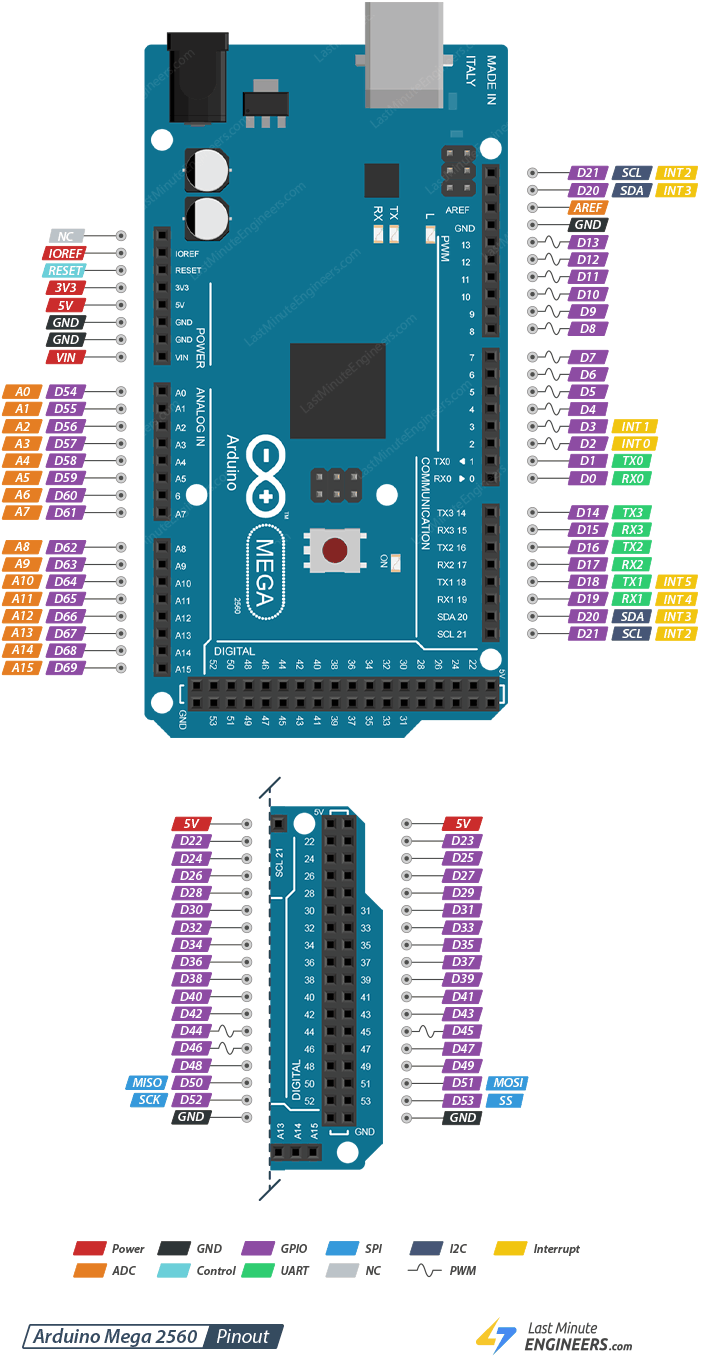
\includegraphics[width=0.75\textwidth]{images/pinout_arduino_mega.png} % Ganti dengan nama file gambar Anda
	\caption{Diagram pemetaan pin (\textit{pinout}) Arduino Mega 2560 (\href{https://lastminuteengineers.com/arduino-mega-pinout/}{Sumber: Last Minute Engineers}).}
	\label{fig:pinout_mega}
\end{figure}

% \subsection{Hubungan Konsep Mikrokontroler dengan Eksplorasi Komponen}
% Pemahaman konseptual mikrokontroler ini menjadi fondasi langsung untuk menganalisis komponen-komponen pada bagian selanjutnya:
% \begin{itemize}
%     \item Konsep **ADC** digunakan untuk menginterpretasikan pembacaan parameter kualitas udara dari sensor MQ-135 dan MQ-2.
%     \item Konsep **GPIO Digital** digunakan untuk membaca luaran biner dari sensor pergerakan HC-SR501 dan sensor jarak FC-51, serta mengendalikan logika aktivasi pada Modul Relay JQC-3FF-S-Z.
%     \item Konsep **PWM dan Timer** digunakan untuk membentuk pewaktuan presisi penentuan sudut pada Servo SG90 serta pengaturan kecepatan putar Motor DC 6V.
% \end{itemize}
